\documentclass[aspectratio=1610]{beamer}
\usetheme{KTH}
\usepackage[utf8]{inputenc}
\usepackage[T1]{fontenc}
\usepackage[format=hang]{caption}
\usepackage{subcaption}
\captionsetup{font=normalsize,labelfont={bf,sf}}
\captionsetup[sub]{font={small}, textfont={normalfont}, labelfont={bf,sf}}
\usepackage{indentfirst}
\usepackage{pgfplots}
\pgfplotsset{compat=1.14}
\usepackage[export]{adjustbox}
\usepackage{tikz}
\usetikzlibrary{shapes,arrows.meta,positioning,automata}
\usepackage{libertine}
\usepackage{sourcecodepro}
\usepackage{todonotes}
\usepackage{wrapfig}

\usepackage[style=ieee,
backend=bibtex,
sorting=none,
sortcites,
maxbibnames=1,
minbibnames=1,
maxcitenames=2, 
mincitenames=1]{biblatex}
\AtBeginBibliography{\footnotesize}
\addbibresource{bibliography.bib}

\newcommand{\kthaffil}{\textsuperscript{\textdagger}}
\newcommand{\cmuaffil}{\textsuperscript{\textdaggerdbl}}

\begin{document}
\startpage
%%%%%%%%%%%%%%%%%%%%%%%%%%%%%%%%%%%%%%%%%%%%%%%%%%%%%%%%%%%%
\begin{frame}{}
    \begin{center}
        \begin{LARGE}
            \textbf{EdgeDroid}\\
        \end{LARGE}
        \emph{An Experimental Approach to Benchmarking Human-in-the-Loop Applications}\\
        \vspace{0.02\textheight}
        {\footnotesize \underline{M. Olguín Muñoz}\kthaffil, J. Wang\cmuaffil, M. Satyanarayanan\cmuaffil and J. Gross\kthaffil\\
            \vspace{0.02\textheight}
            \kthaffil~KTH Royal Institute of Technology, Sweden\hspace{.1\linewidth}\cmuaffil~Carnegie Mellon University\\}
    \end{center}

    \vspace{0.04\textheight}

    \begin{tiny}
        \raggedleft%
        \emph{HotMobile'19 Session 5: February 28\textsuperscript{th} 2019, Santa Cruz, CA}\\
    \end{tiny}
\end{frame}

\normalpage%
{
    % within group to not have an outline for the first section
    \AtBeginSection[]{}
    \section{Introduction}
}

\begin{frame}{}
    \begin{center}
        \begin{tikzpicture}[align=center, every node/.style={inner sep=0pt, anchor=center}]

    % central image
    \node[visible on= <2->] (user) {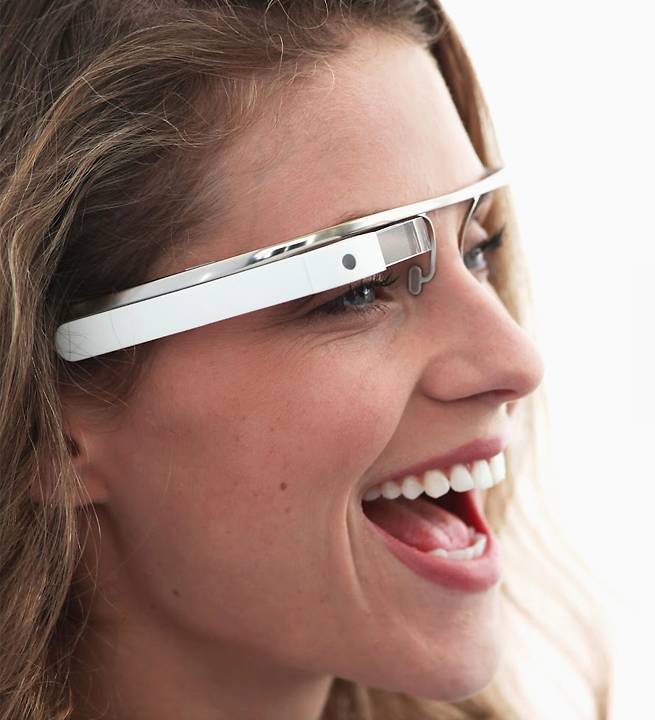
\includegraphics[height=.2\textheight]{img/google-glass.png}};
    \node [right=6em of user, visible on= <2->] (server) {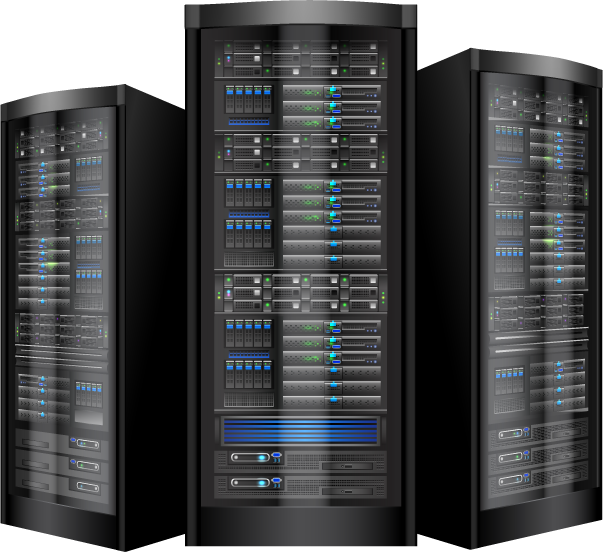
\includegraphics[height=.2\textheight]{img/server.png}};
    \path (user) -- coordinate[midway] (center) (server);

    % surrounding images
    \node[left=1em of user] (pokemon) {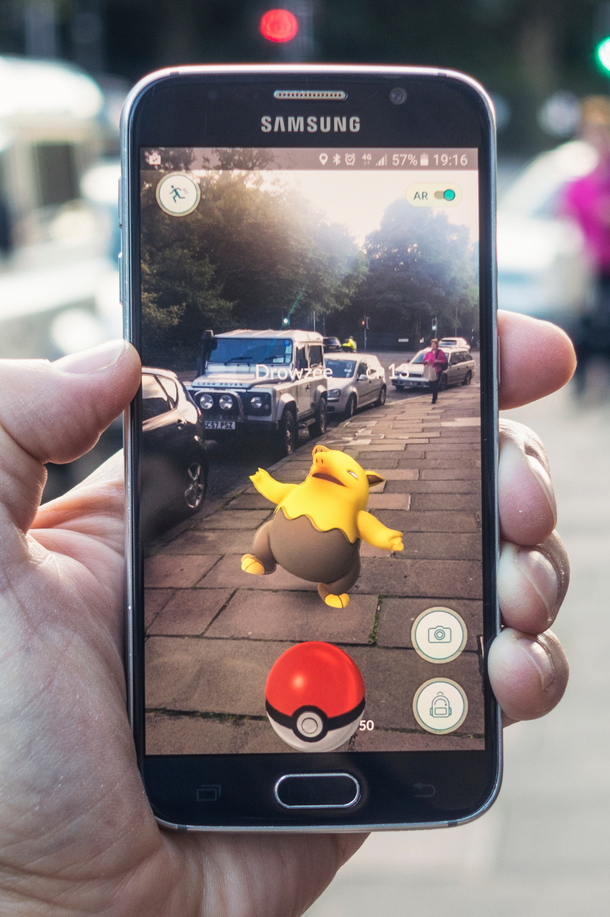
\includegraphics[height=.3\textwidth]{img/ar_pokemongo.jpg}};
    \node[right=1em of server] (ar) {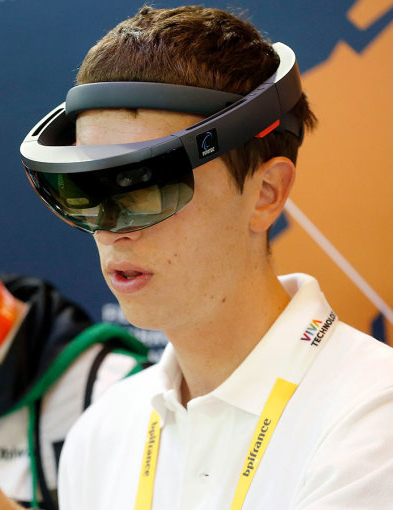
\includegraphics[height=.3\textwidth]{img/augmentedreality.jpg}};
    \node[above=5em of center] (hud) {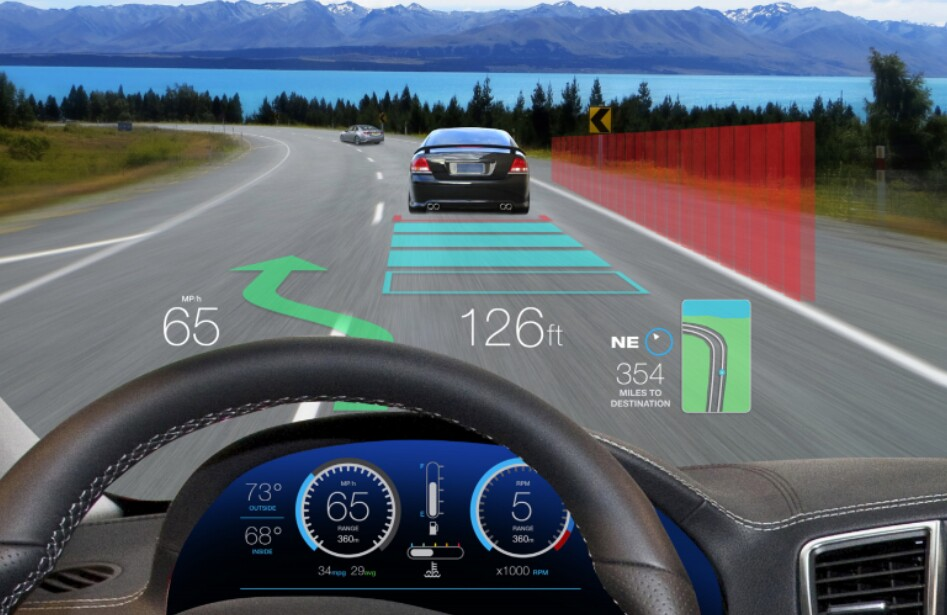
\includegraphics[height=.25\textheight]{img/AR_HUD_proc.jpg}};
    \node[below=7em of center] (glass) {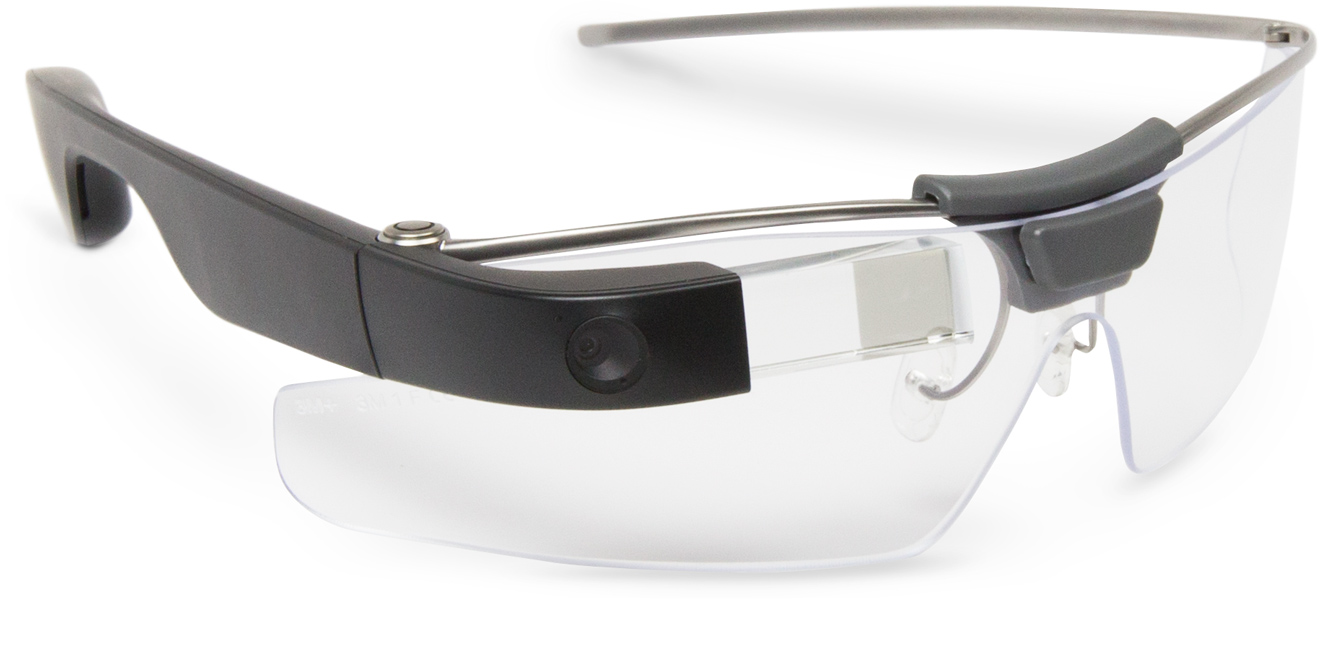
\includegraphics[height=.2\textheight]{img/glass_wearable.jpeg}};


    \path[draw, -{Latex[length=2mm]}, very thick, visible on= <2->]
    (user) edge [out=45, in=135] node[above] {Sensory Input} (server)
    (server) edge [out=225, in=315] node[below] {Human-parseable\\Feedback} (user);
\end{tikzpicture}\\
    \end{center}
\end{frame}

% \begin{frame}{Human-in-the-Loop Applications}
%     \begin{columns}[onlytextwidth]
%         \begin{column}{.5\linewidth}
%             $\left.
%             \begin{tabular}{p{.85\linewidth}}
%                 \begin{itemize}
%                     \itemsep2em
%                     \item Application Developers
%                     \onslide<2->{\begin{itemize}
%                         \item Debugging
%                         \item Resource Consumption
%                         \item Performance and Optimization
%                     \end{itemize}}
%                     \item Infrastructure Providers
%                     \onslide<3->{\begin{itemize}
%                         \item Performance and Optimization
%                         \item Scaling
%                     \end{itemize}}
%                     \item Researchers
%                 \end{itemize}
%             \end{tabular}
%             \right\}$
%         \end{column}
%         \begin{column}{.5\linewidth}
%             \centering\Large\bfseries%
%             \onslide<4->{How to obtain these measurements?}
%         \end{column}
%     \end{columns}
%     \todo[inline]{Too much text?}
% \end{frame}

\begin{frame}{Studying Human-in-the-Loop Applications}
    Need to understand and optimize these applications:% and the underlying infrastructure:
    \begin{itemize}
        \item How do they interact with each other?
        \item How do they interact with infrastructure?
        \item How do they scale?
        %\item KPI: Delays, Round-Trip Times (RTTs).
    \end{itemize}%
    \vspace{1em}%
    \begin{center}
        {\Large With which methodology can we study these behaviors?}\\
        \vspace{2em}%
        \begin{tikzpicture}[align=center,
    arrow/.style={draw, very thick, line cap=round, -{Latex[length=2.5mm]}},
    arrowr/.style={arrow, {Latex[length=2.5mm]}-},
    userimg/.style={inner sep=0mm, label={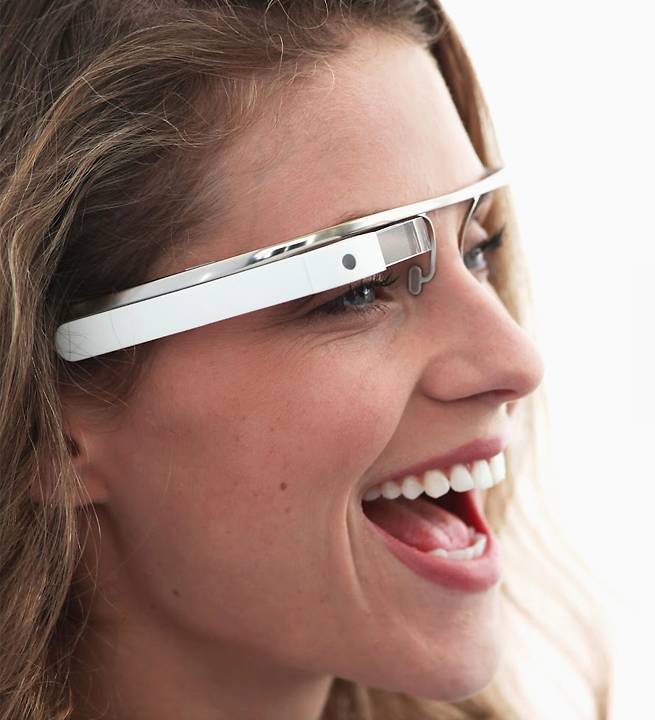
\includegraphics[height=.07\textheight]{img/google-glass.png}}}]


    \node [inner sep=0pt, visible on= <1>] (user) {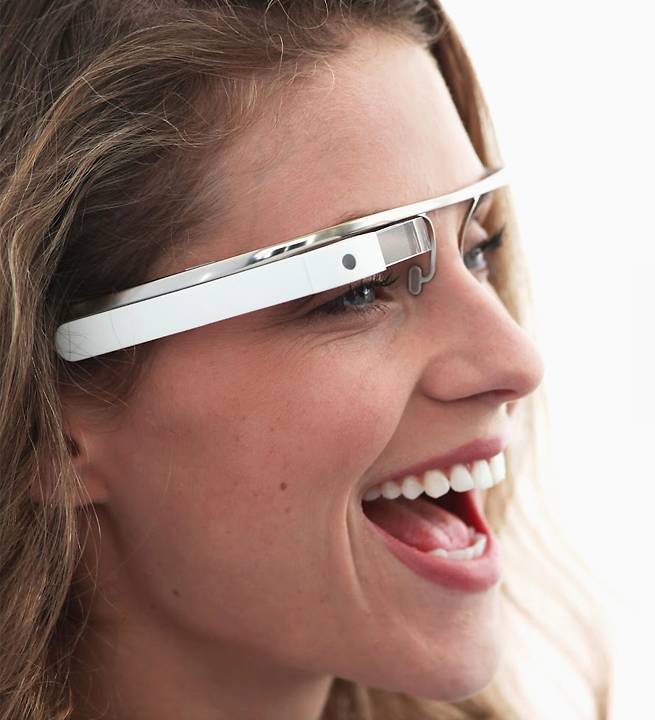
\includegraphics[height=.2\textheight]{img/google-glass.png}};
    \node [inner sep=0pt, right=4em of user] (server) {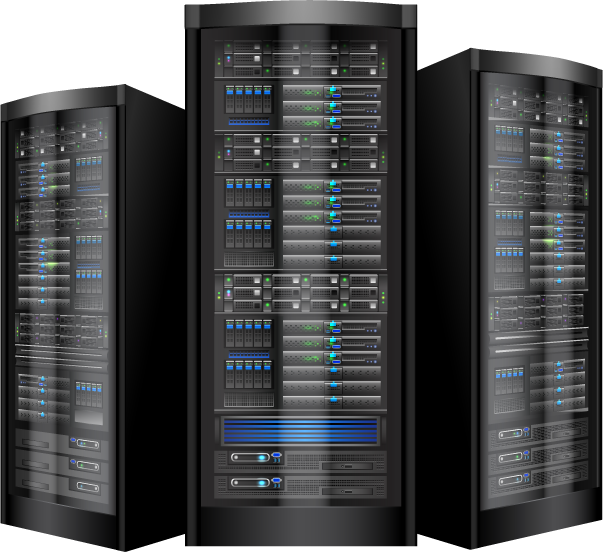
\includegraphics[height=.2\textheight]{img/server.png}};
    
    \matrix [inner sep=0mm, column sep=0mm, row sep=0mm, visible on= <2->, anchor=east] (mtx) at (user.east) {
        \node[userimg] {}; & \node[userimg] {}; & \node[userimg] {}; & \node[userimg] {}; 
        & \node[userimg] {}; & \node[userimg] {}; & \node[userimg] {}; & \node[userimg] {}; \\

        \node[userimg] {}; & \node[userimg] {}; & \node[userimg] {}; & \node[userimg] {}; 
        & \node[userimg] {}; & \node[userimg] {}; & \node[userimg] {}; & \node[userimg] {}; \\

        \node[userimg] {}; & \node[userimg] {}; & \node[userimg] {}; & \node[userimg] {}; 
        & \node[userimg] {}; & \node[userimg] {}; & \node[userimg] {}; & \node[userimg] {}; \\
    };

    \draw[arrow, visible on= <1>] (server.170) -- (server.170 -| user.east);
    \draw[arrowr, visible on= <1>] (server.190) -- (server.190 -| user.east);

    \draw[arrow, visible on= <2->] (server.170) -- (server.170 -| mtx.east);
    \draw[arrowr, visible on= <2->] (server.190) -- (server.190 -| mtx.east);

    % big dollar sign
    \node[inner sep=0mm, anchor=center, visible on= <3->] at (mtx.center) {
\includegraphics[height=.15\textheight]{img/dollar.png}};

\end{tikzpicture}\\
        \Large\bfseries\color{red}\onslide<3->{Costly}\onslide<4->{, poor repeatability\\}
        %\onslide<5->{Require IRB approval!\\}
    \end{center}
\end{frame}

\section{Background}
\begin{frame}{Previous \& Related Work}
    \begin{center}
        \begin{tikzpicture}[align=center, every node/.style={inner sep=2mm, circle, draw, very thick, text width=5em}]

    \matrix[inner sep=0pt, column sep=4em, row sep=0pt, draw=none, rectangle] (mtx) {
        \node[fill=C1, font=\color{white}] (proto) 
        {Prototyping\\\autocite{Ha:TowardsWearableCogAssist,Chen:EarlyImplementation,Chatzopoulos:Hyperion}};
        & \node[fill=C4, font=\color{white}] (latency) 
        {Latencies\\\autocite{Chen:AnEmpiricalStudyOfLatency}};
        & \node[fill=C5, font=\color{white}] (models) 
        {Models\\\autocite{Zubaidy15,Schiessl17}};
        \\
    };
\end{tikzpicture}\\
    \end{center}
    \onslide<2->{%
        \begin{block}{Our Contributions}
            \begin{itemize}
                \item A methodology for benchmarking human-in-the-loop applications.
                      \onslide<3->{\item EdgeDroid: A benchmarking tool-suite.}
                      \onslide<4->{\item Experiments and measurements which show the effectiveness of the approach.}
            \end{itemize}
        \end{block}%
    }
\end{frame}

\section{EdgeDroid: Experimentally Benchmarking Human-in-the-Loop}

\begin{frame}{Approach}
    \begin{center}
        \begin{tikzpicture}[align=center]

    \node[inner sep=2.6mm, draw, circle, fill=white!80!blue, visible on= <3>] 
    (user) {User\\Model};
    \node[inner sep=0pt, anchor=center, left=4em of user, visible on= <3>] 
    (trace) {
\includegraphics[height=.12\textheight]{img/floppy.png}\\Trace};

    \node [inner sep=0pt, anchor=center, right=8em of user] 
    (server) {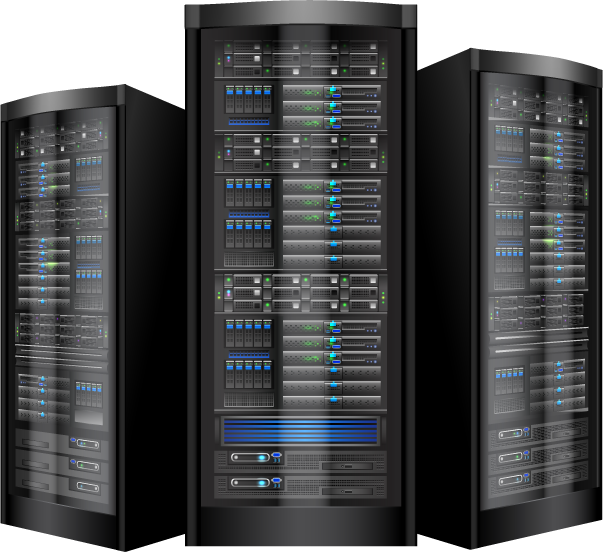
\includegraphics[height=.2\textheight]{img/server.png}};
    
    \coordinate[below=3em of server] (serverarrowanchor) {};

    \draw[very thick, line cap=round, -{Latex[length=2.5mm]}, visible on= <3>] 
    (user.east) -- coordinate[midway, above] (inputlabelcoord) (server.west);

    \draw[very thick, line cap=round, -{Latex[length=2.5mm]}, visible on= <3>]
    (trace.east) -- (user.west);

    \draw[very thick, line cap=round]
    (server.south) -- (serverarrowanchor);

    \draw[very thick, line cap=round, -{Latex[length=2.5mm]}, visible on= <3>]
    (serverarrowanchor) -| (user.south);

    \node[inner sep=0pt, anchor=base, above=1mm of inputlabelcoord] (inputlabel) {Inputs};
    \node[inner sep=0pt, anchor=base, below=18mm of inputlabel] (feedbacklabel) {Feedback};

    \node[fit=(server) (feedbacklabel) (serverarrowanchor), draw, rectangle, dashed, inner sep=1em] (fitbackend) {};
    \node[inner sep=0mm, anchor=base, above=2mm of fitbackend.north] (fitbackendlabel) {Real backend \& network};

    \node[fit=(trace) (user) (user.south |- serverarrowanchor), draw, rectangle, dashed, inner sep=1em] (fituser) {};
    \node[inner sep=0mm, anchor=base, above=2mm of fituser.north, visible on= <3>] (fituserlabel) {Emulated user};

    % real user shit
    \node[inner sep=0mm, anchor=center, visible on= <1-2>] 
    (realuser) at (fituser.center) {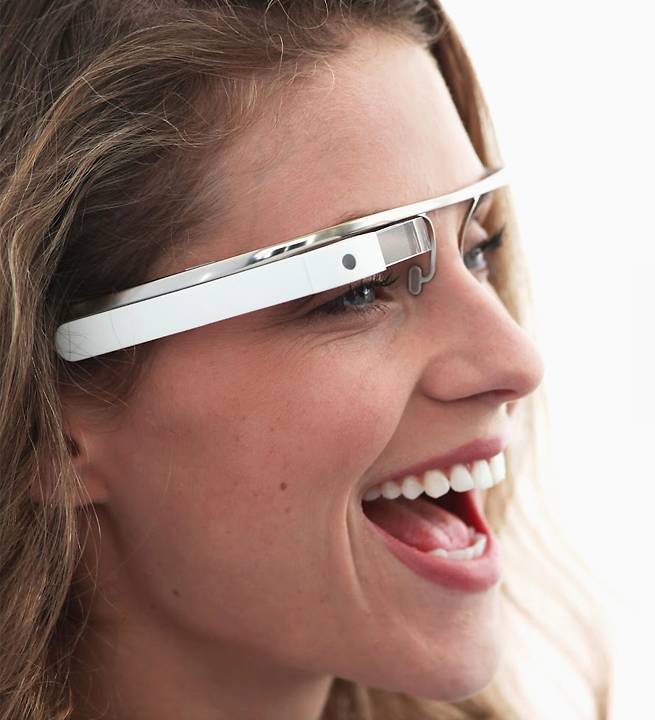
\includegraphics[height=.2\textheight]{img/google-glass.png}};
    \node[inner sep=0mm, anchor=base, above=2mm of fituser.north, visible on= <1-2>] 
    (realuserlabel) {Real user};

    \draw[very thick, line cap=round, {Latex[length=2.5mm]-}, visible on= <1-2>] 
    (server.west) -- (server.west -| realuser.east);
    \draw[very thick, line cap=round, -{Latex[length=2.5mm]}, visible on= <1-2>]
    (serverarrowanchor) -| (realuser.south);

    \draw[red, line width=2mm, line cap=round, visible on= <2>]
    (realuser.south west) -- (realuser.north east)
    (realuser.south east) -- (realuser.north west);

\end{tikzpicture}\\%
        \vspace{.1\textheight}%
        \only<1>{%
            Benchmarking human-in-the-loop applications is HARD\\%
        }%
        \only<2->{What if we could do away with the human users?\\}%
        \onslide<3->{\bfseries\color{red}Repeatable, scalable!\\}%
        %\onslide<4->{\vspace{.05\textheight}Key question: Credibility.\\}
    \end{center}
\end{frame}

\begin{frame}{Example: Task Guidance WCA, LEGO Assistant\ \autocite{Ha:TowardsWearableCogAssist}}
    \begin{center}
        \begin{tikzpicture}[align=center, arrow/.style={very thick, line cap=round, -{Latex[length=2.5mm]}}, font=\footnotesize]
    \matrix[inner sep=0pt, column sep=4em, row sep=0pt] (mtx1) {
        \node[inner sep=0pt] (step0) {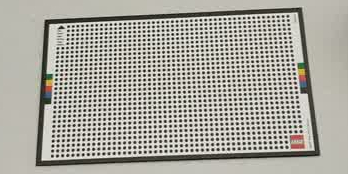
\includegraphics[height=.2\textheight]{img/lego/img0.jpeg}};
        & \node[inner sep=0pt] (step1) {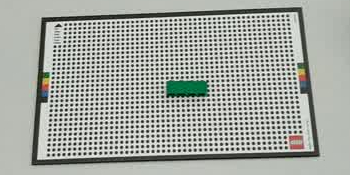
\includegraphics[height=.2\textheight]{img/lego/img1.jpeg}};\\
    };

    \node[inner sep=2mm, text width=11em, draw, rectangle, very thick, below=3em of mtx1] 
    (instruction) {Example instruction:\\``Put the white 1x1 brick on top of the green 1x4 brick.''};

    \matrix[inner sep=0pt, column sep=4em, row sep=0pt, below=3em of instruction] (mtx2) {
        \node[inner sep=0pt] (step2) {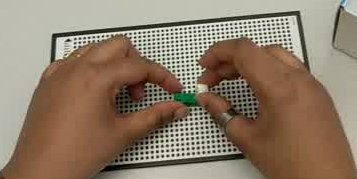
\includegraphics[height=.2\textheight]{img/lego/img2.jpeg}};
        & \node[inner sep=0pt] (step3) {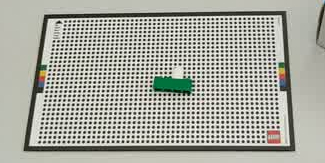
\includegraphics[height=.2\textheight]{img/lego/img3.jpeg}};\\
    };

    \coordinate[right=2em of step1.east] (a1);
    \coordinate[left=2em of step2.west] (a2);

    \begin{scope}[arrow]
        \draw (step0) -- node[midway, above, sloped] {\Large\ldots} (step1);
        \draw (step2) -- node[midway, above, sloped] {\Large\ldots} (step3);
        \draw (a1) |- (instruction);
        \draw (a2) -- (step2);
    \end{scope}

    \begin{scope}[very thick, line cap=round]
        \draw (step1) -- (a1);
        \draw (instruction) -| (a2);
    \end{scope}

    \node[fit=(step0) (step1), draw, rectangle] (fit1) {};
    \node[fit=(step2) (step3), draw, rectangle] (fit2) {};

    \node[inner sep=0mm, below=1mm of fit1.south] (label1) {Step $N$};
    \node[inner sep=0mm, above=1mm of fit2.north] (label2) {Step $N+1$};

\end{tikzpicture}\\
        %\vspace{.2\textheight}%
        %\begin{tikzpicture}[align=center, font=\tiny\bfseries,
    %node styles:
    block_center/.style ={rectangle, draw=black, thick, fill=white,
            text width=6em, text centered, minimum height=2em, inner sep=1mm},
    block_rounded/.style ={rectangle, draw=black, thick, fill=white, inner sep=1mm,
            text width=6em, text centered, rounded corners=.55cm, minimum height=2em},
    arrow/.style={draw, thick, -{Latex[length=2mm]}},
    arrowr/.style={draw, thick, {Latex[length=2mm]}-}
    ]

    \matrix [column sep=10mm,row sep=3mm, inner sep=0mm] (top) {
        \node [block_center] (detect) {Detection};
         & \node [block_center] (repr) {Symbolic\\Repr.};
         & \node [block_center] (model) {Task Model\\$M\{S, E\}$};
         & \node [block_center] (feedback) {Feedback\\Generation}; \\[3ex]
    };

    \matrix [column sep=10mm,row sep=3mm, below=1mm of top, inner sep=0mm] (bottom) {
        \node [block_rounded] (sensors) {On-body\\Sensors};
         & \node[maninblack, minimum height=4em] (user) {Human User};
         & \node [block_rounded] (hud) {HUD, Speakers,\\etc.}; \\
    };

    %\Smiley[1, below of=bottom] (smiley);


    \begin{scope}[every path/.style=arrow]
        \path (detect) -- (repr);
        \path (repr) -- (model);
        \path (model) -- (feedback);
        \path (feedback.south) |- (hud);
        \path (hud) -- (hud -| user.east);
        \path (sensors.west) -| (detect);
    \end{scope}

    \begin{scope}[every path/.style=arrowr]
        \path (sensors) -- (sensors -| user.west);
    \end{scope}

\end{tikzpicture}\\%
    \end{center}
\end{frame}

\begin{frame}{Tracing}
    \begin{center}
        \begin{tikzpicture}[align=center, node distance=0.7cm and 0.7cm,
    line/.style ={draw, very thick, line cap=round, -{Latex[length=2.5mm]}, shorten >=0pt}]
    \matrix [column sep=4mm,row sep=10mm] (mtx) {
        & \node[draw, circle, minimum height=17mm, fill=white!60!red,
            minimum width=17mm, anchor=center] (record) {Recorder};
        & \node[inner sep=0pt] (trace) {
\includegraphics[height=.12\textheight]{img/floppy.png}\\Trace}; \\


        \node[inner sep=0pt] (user) {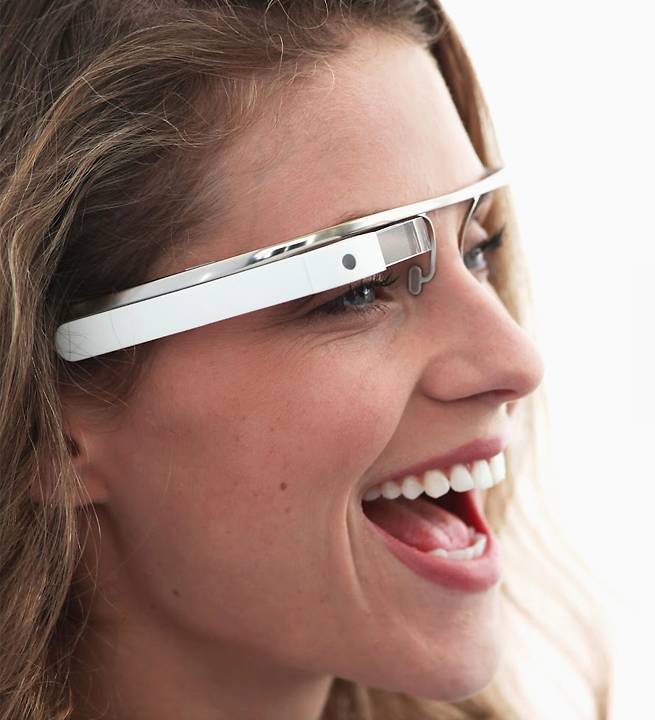
\includegraphics[height=.2\textheight]{img/google-glass.png}};
         & \node[draw=black, fill=white!80!orange, thick, single arrow, minimum height=33mm,
            minimum width=16mm, single arrow head extend=2mm, anchor=center] (inputs) {Sensory inputs};
         & \node [inner sep=0pt] (server) {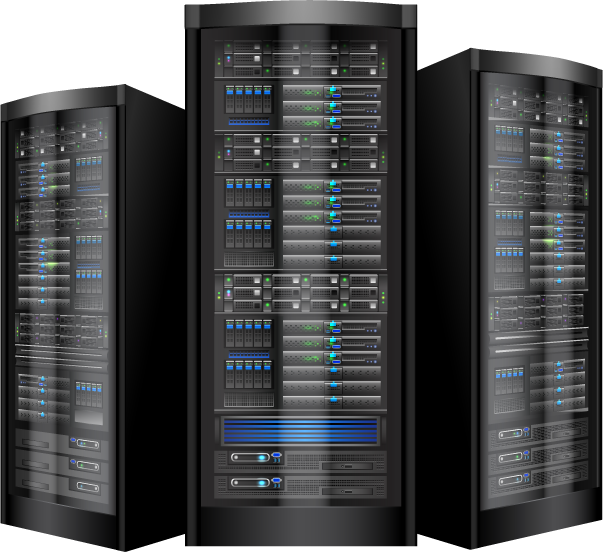
\includegraphics[height=.2\textheight]{img/server.png}}; \\
    };

    \path[draw, line]
    (record) edge node {} (trace)
    (inputs) edge node {} (record);

    %\draw[thick, line cap=round, -{Latex[length=2.5mm]}, shorten >=0pt]
    %(record.east) -- (trace.west);


    %(inputs.north) -- (record.south);

    %\draw[white!30!violet, line width=.5mm, line cap=round]
    %(inputs.160) -- (record.225)
    %(inputs.20) -- (record.315);
\end{tikzpicture}\\
        \vspace{.1\textheight}%
        \begin{tikzpicture}[align=center]
    
    \matrix[inner sep=0mm, column sep=1em, row sep=0mm] (mtx) {
        \node[inner sep=0pt, anchor=center] (trace) {
\includegraphics[height=.12\textheight]{img/floppy.png}}; 
        & 
        & \node[inner sep=0pt, anchor=center] (lego0) {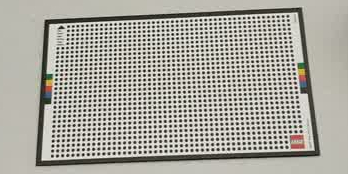
\includegraphics[height=.12\textheight]{img/lego/img0.jpeg}}; 
        & \node[inner sep=0pt, anchor=center] (lego1) {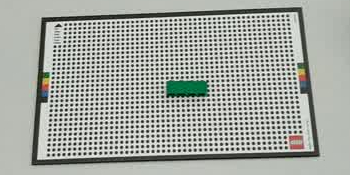
\includegraphics[height=.12\textheight]{img/lego/img1.jpeg}}; 
        & \node[inner sep=0pt, anchor=center] (lego2) {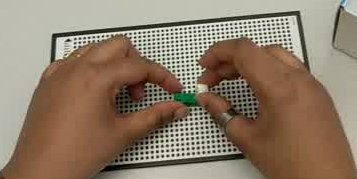
\includegraphics[height=.12\textheight]{img/lego/img2.jpeg}}; 
        & \node[inner sep=0pt, anchor=center] (lego3) {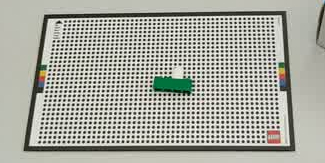
\includegraphics[height=.12\textheight]{img/lego/img3.jpeg}}; 
        \\
    };

    \node[fit=(lego0) (lego1) (lego2) (lego3), very thick, draw, rectangle] (fit) {};

    \begin{scope}[very thick, line cap=round]
        \draw (trace.east) -- (fit.north west);
        \draw (trace.east) -- (fit.south west);
    \end{scope}

\end{tikzpicture}\\
    \end{center}
\end{frame}

\begin{frame}{Trace Replay}
    \onslide<1->{\begin{block}{Non-trivial Challenge}
            \begin{itemize}
                \item Changes in system responsiveness require adapting trace.
                \item System delays affect user behavior as well.
            \end{itemize}
        \end{block}}
    \onslide<2->{\begin{block}{Our Approach}
            \begin{itemize}
                \item Segment trace into logical ``steps''.
                \item Controlled replay of steps.
                %\item Future work: model of user behavior.
            \end{itemize}
        \end{block}
        \begin{center}
            \begin{tikzpicture}[align=center]

    \node[inner sep=2.6mm, draw, circle, fill=white!80!blue] (user) {User\\Model};
    \node [inner sep=0pt, anchor=center, right=8em of user] (server) {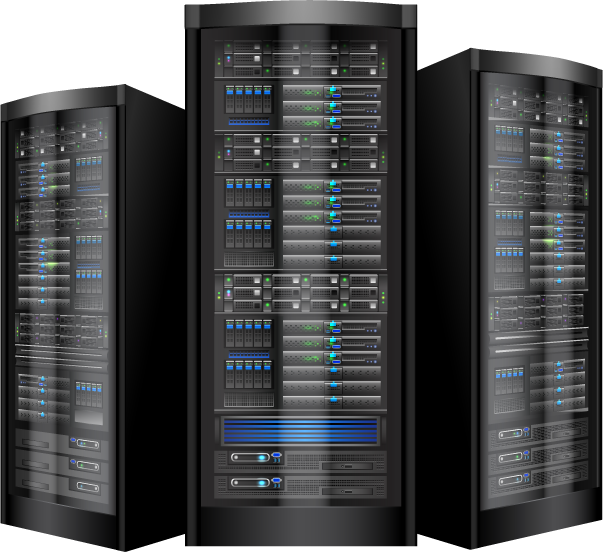
\includegraphics[height=.2\textheight]{img/server.png}};
    \node[inner sep=0pt, anchor=center, left=4em of user] (trace) {
\includegraphics[height=.12\textheight]{img/floppy.png}};

    \coordinate[below=3em of server] (serverarrowanchor) {};

    \draw[very thick, line cap=round, -{Latex[length=2.5mm]}] 
    (user.east) -- node[midway, above] (inputlabel) {Inputs} (server.west);

    \draw[very thick, line cap=round, -{Latex[length=2.5mm]}]
    (trace.east) -- (user.west);

    \draw[very thick, line cap=round]
    (server.south) -- (serverarrowanchor);
    \draw[very thick, line cap=round, -{Latex[length=2.5mm]}]
    (serverarrowanchor) -| (user.south); 
    \node[inner sep=0pt, anchor=center, below=16mm of inputlabel] (feedbacklabel) {Feedback};

    \node[fit=(server) (feedbacklabel) (serverarrowanchor), draw, rectangle, dashed, inner sep=1em] (fitbackend) {};
    \node[inner sep=0mm, anchor=base, above=2mm of fitbackend.north] (fitbackendlabel) {Real backend \& network};

    \node[fit=(trace) (user) (user.south |- serverarrowanchor), draw, rectangle, dashed, inner sep=1em] (fituser) {};
    \node[inner sep=0mm, anchor=base, above=2mm of fituser.north] (fituserlabel) {Emulated user};

\end{tikzpicture}\\
        \end{center}}
\end{frame}

\begin{frame}{Implementation}
    \begin{center}
        \begin{tikzpicture}[align=center, font={\footnotesize},
    arrow/.style={draw, thick, -{Latex[length=2mm]}},
    arrowr/.style={draw, thick, {Latex[length=2mm]}-},
    parallelogram/.style={trapezium,trapezium left angle=70,trapezium right angle=-70}]

    % layers
    \pgfdeclarelayer{background0}
    \pgfdeclarelayer{background1}
    \pgfdeclarelayer{foreground}
    \pgfsetlayers{background0,background1,foreground}
    
    \begin{pgfonlayer}{foreground}
        \matrix[column sep=40mm, row sep=2mm, inner sep=2mm,
        every node/.style={text width=4em, text centered, minimum width=5em}] (mtx) {
            \node[dashed, draw, rectangle, anchor=center, inner sep=2mm, ] (usermodel) {``User''\\Model}; 
            & \node[draw, dashed, rectangle, anchor=center, inner sep=2mm] (app_backend) {App Backend};\\

            \node[inner sep=0mm] {}; %spacer
            & \node[anchor=center, inner sep=0mm] (docker) {Container};\\

            % spacers
            \node[inner sep=0mm, minimum height=1.5em] {};
            & \node[inner sep=0mm, minimum height=1.5em] {}; \\

            \node[anchor=center, inner sep=2mm, minimum height=5em] (emulator) {Client Emulator\\Java 1.8};
            & \node[anchor=center, inner sep=2mm, minimum height=5em] (control) {Control Backend\\Python 3.6};\\

            % spacers
            \node[inner sep=0mm, minimum height=.5em] {};
            & \node[inner sep=0mm, minimum height=.5em] {}; \\

            \node[inner sep=0mm, minimum height=2em] (label1_padding) {}; 
            & \node[inner sep=0mm, minimum height=2em] (label2_padding) {}; \\
        };

        \node[parallelogram, draw, inner sep=2mm, right=10mm of control.25, 
        minimum width=20mm, minimum height=2em, fill=white!80!violet] (config) {Config};
        \node[parallelogram, draw, inner sep=2mm, right=10mm of control.335, 
        minimum width=20mm, minimum height=2em, fill=white!80!violet] (trace) {Trace};
    \end{pgfonlayer}

    \begin{pgfonlayer}{background1}
        \node[fit=(usermodel) (emulator), draw, fill=white!80!yellow] (fit1) {};
        %\node[fit=(app_backend) (control)] (fit2) {};
        \node[fit=(docker) (app_backend), draw, fill=white!80!blue] (fit3) {};
        \node[fit=(control), draw, fill=white!80!red] (fit_control) {}; % just to make the size match
    \end{pgfonlayer}

    % main background fits
    \begin{pgfonlayer}{background0}
        \node[fit=(label1_padding) (fit1), draw, fill=white!80!green] (android) {};
        \node[fit=(label2_padding) (fit_control) (fit3) (config.top right corner) (trace.top right corner), draw, fill=white!80!black] (cloudlet) {};
    \end{pgfonlayer}

    \begin{pgfonlayer}{foreground}
        % primary labels
        \node[inner sep=2mm, above] at (android.south) {Android\\6.0+};
        \node[inner sep=2mm, above] at (cloudlet.south) {Cloudlet\\Linux v4.13.0+};


        % arrows
        % config and trace
        \draw[arrow] (config.west) -- (config.west -| fit_control.east);
        \draw[arrow] (trace.west) -- (trace.west -| fit_control.east);

        % between app and control backend
        \draw[arrowr] (fit_control.95) -- (fit_control.95 |- fit3.south);
        \draw[arrow] (fit_control.85) -- node[right] {\footnotesize Execution Control} (fit_control.85 |- fit3.south);

        % between app and user model
        \coordinate (a1) at (app_backend.165 -| fit3.west);
        \coordinate (a2) at (app_backend.195 -| fit3.west);
        \coordinate (b1) at (a1 -| fit1.east);
        \coordinate (b2) at (a2 -| fit1.east);

        \draw[arrow] (a1) -- coordinate[midway] (ab1) (b1);
        \draw[arrowr] (a2) -- coordinate[midway] (ab2) (b2);
        \path (ab1) -- node[midway, anchor=center, inner sep=0mm] {Feedback Loop} (ab2); % center label between arrows

        % between control and client
        \draw[arrow, dashed] (fit_control.155) -- node[above] {Config, Trace} node[below] {\tiny Before experiment} (fit_control.155 -| fit1.east);
        \draw[arrowr, dashed] (fit_control.205) -- node[above] {Results} node[below] {\tiny After experiment} (fit_control.205 -| fit1.east);
    \end{pgfonlayer}

\end{tikzpicture}\\
        \vspace{.1\textheight}
        \Large\icontag{\faGithub}{\urlref{https://github.com/molguin92/EdgeDroid}}
    \end{center}
\end{frame}

\begin{frame}{Evaluation}
    \begin{center}
        \Large%
        \textbf{Key purpose:}\\
        Demonstrate utility of EdgeDroid.\\
    \end{center}
\end{frame}

\begin{frame}{Evaluation: Setup}
    \begin{columns}[onlytextwidth]
        \begin{column}{.5\linewidth}
            \begin{block}{Application \& Scenarios}
                \begin{center}
                    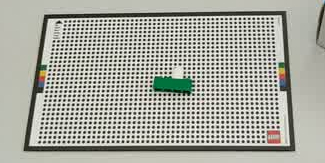
\includegraphics[width=.7\linewidth]{img/lego/img3.jpeg}

                    LEGO Assistant
                \end{center}
                \begin{itemize}
                    \item Three \emph{optimal} scenarios with 1, 5 and 10 devices.
                    \item Weakened wireless link with 10 devices.
                    \item KPI: Round-Trip Time (RTT).
                \end{itemize}
            \end{block}%
        \end{column}%
        \begin{column}{.5\linewidth}
            \raggedleft%
            \begin{tikzpicture}[grow'=right, font=\footnotesize]
                \tikzset{level distance=6em, sibling distance=1em}
                \tikzset{every tree node/.style={anchor=center}}
                \Tree [.\node[] {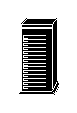
\includegraphics[width=.1\linewidth]{img/symbols/tower}};
                \edge[] node[above, sloped] {Ethernet}; [.\node[] {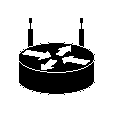
\includegraphics[width=.1\linewidth]{img/symbols/router}};
                \edge[dashed]; \node[] {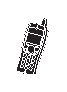
\includegraphics[width=.1\linewidth]{img/symbols/cellphone}};
                \edge[dashed]; \node[] {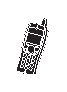
\includegraphics[width=.1\linewidth]{img/symbols/cellphone}};
                \edge[color=white] node[midway, color=black, inner sep=0mm] {WiFi}; \node[inner sep=0mm] {};
                \edge[dashed]; \node[] {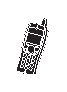
\includegraphics[width=.1\linewidth]{img/symbols/cellphone}};
                \edge[dashed]; \node[] {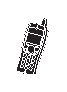
\includegraphics[width=.1\linewidth]{img/symbols/cellphone}};
                ] ];
            \end{tikzpicture}
        \end{column}%
    \end{columns}
\end{frame}

\begin{frame}{Use Cases}
    \begin{center}
        \begin{tikzpicture}[align=center, font={\footnotesize}]

    \matrix[inner sep=0pt, column sep=3em, row sep=1em, ampersand replacement=\nextcell] (mtx) {

        \node[inner sep=0pt] (r1) {State change vs. no state change.\\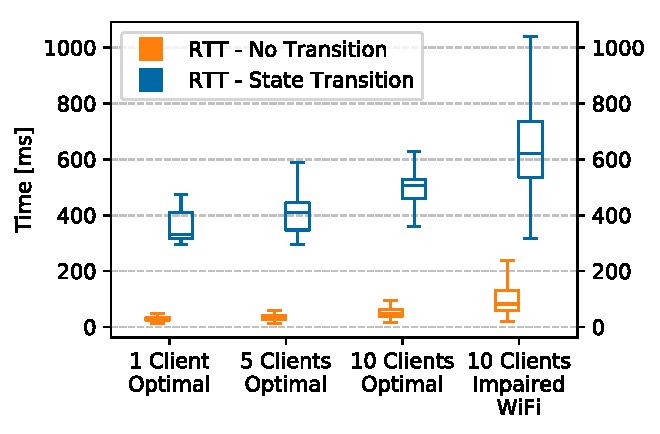
\includegraphics[width=.42\linewidth]{plots/rtt_fb_vs_nofb.pdf}};
        \nextcell \node[inner sep=0pt] (r2) {Times by pipeline segments.\\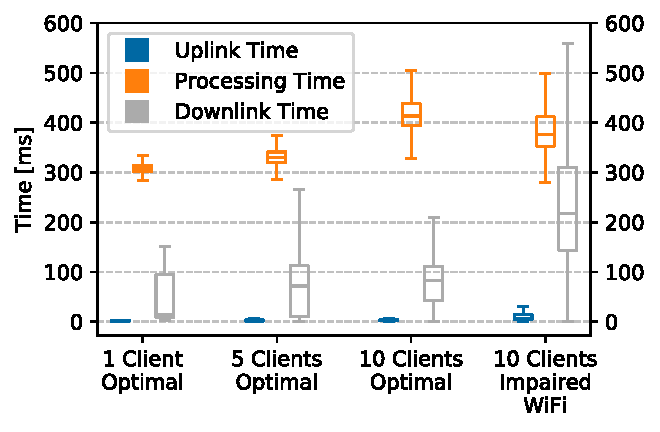
\includegraphics[width=.42\linewidth]{plots/box_feedback.pdf}}; \\

        \node[inner sep=0pt] (r3) {RTT by task step.\\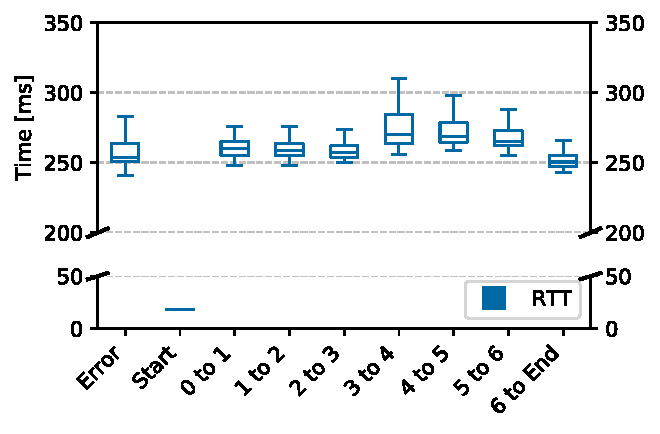
\includegraphics[width=.42\linewidth]{plots/box_taskstep.pdf}};
        \nextcell \node[inner sep=0pt] (r4) {%
        %Reference latency bounds for LEGO\\(\textcite{Chen:AnEmpiricalStudyOfLatency})\\
        %\ \\
        %\begin{tabular}{@{}ll@{}}
        %    \toprule
        %    Latency {[}ms{]} & Quality   \\ \midrule
        %    $< 600$          & Excellent \\
        %    $600-2700$       & Impaired  \\
        %    $> 2700$         & Unusable  \\ \bottomrule
        %\end{tabular}%
        }; \\
    };

\end{tikzpicture}\\
    \end{center}
\end{frame}

\section{Conclusions}
\begin{frame}{Conclusions}
    \begin{block}{Future Work}
        \begin{itemize}
            \item User Model.
            \item Other types of Applications.
        \end{itemize}
    \end{block}

    \begin{block}{Summary}
        \begin{itemize}
            \item Need to study the scaling of Human-in-the-Loop applications.
                  \begin{itemize}
                      \item Difficult due to human users.
                  \end{itemize}
            \item Methodology + tool suite for benchmarking:
                  \begin{itemize}
                      \item \textbf{EdgeDroid}
                      \item Trace based.
                      \item Model of human behavior.
                  \end{itemize}
            \item Results which show the utility of EdgeDroid.
        \end{itemize}
    \end{block}
\end{frame}

\startpage
\begin{frame}{}
    \begin{center}
        \textbf{\Large Thank you.}\\
        \vspace{.1\textheight}%
        \begin{block}{\footnotesize Contact}
            \tiny%
            \textbf{Manuel Olguín Muñoz}\\
            Division of Information Science and Engineering\\
            KTH EECS\\
            Malvinas väg 10, 100-44 Stockholm, SWEDEN\\
            \vspace{.01\textheight}
            Email: \emailref{molguin@kth.se}\\
            Website: \urlref{https://olguin.se}\\
        \end{block}
    \end{center}
    \vspace{.1\textheight}%
\end{frame}

\normalpage
\section{Extra Slides}
\begin{frame}{Requirements}
    \begin{columns}[onlytextwidth]
        \begin{column}{.5\linewidth}
            $\left.
                \begin{tabular}{p{.8\linewidth}}
                    \begin{itemize}
                        \itemsep2em
                        \item Generate realistic, high-dimensional, real-time inputs.
                        \item Correctly and realistically react to feedback.
                        \item KPI: Delays.
                    \end{itemize}
                \end{tabular}%
                \right\}$
        \end{column}%
        \begin{column}{.5\linewidth}
            \centering%
            \Large\bfseries%
            Trace of pre-recorded inputs\\
            \& a model of user behavior\\
        \end{column}
    \end{columns}
\end{frame}

\begin{frame}{User Model}
    \begin{center}
        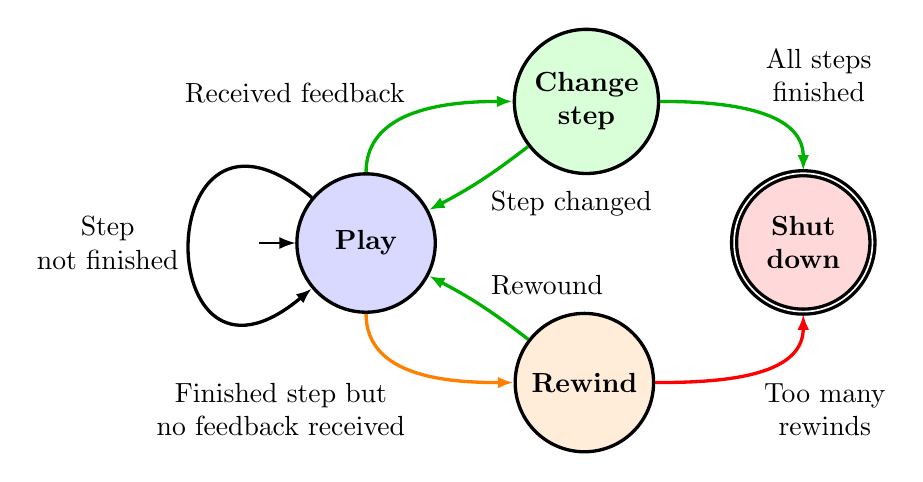
\begin{tikzpicture}[align=center,
    node distance=.5cm and 1.5cm,
    every initial by arrow/.style={-{Latex[length=2mm]}}]
    % Place nodes              
    \node [initial, very thick, state, minimum size=5em, initial text=, fill=white!85!blue] (play) {\textbf{Play}};
    \node [state, very thick, above right=of play, minimum size=5em, fill=white!85!green] (change) {\textbf{Change}\\\textbf{step}};
    \node [state, very thick, below right=of play, minimum size=5em, fill=white!85!orange] (rewind) {\textbf{Rewind}};
    \node [state, very thick, accepting, above right=of rewind, minimum size=5em, fill=white!85!red] (shutdown) {\textbf{Shut}\\\textbf{down}};

    % Draw edges
    \path[draw, -{Latex[length=2mm]}, very thick]
    (play) edge [out=270, in=180, color=red!50!yellow] node[below left, color=black] {Finished step but\\no feedback received} (rewind)
    edge [out=90, in=180, color=black!30!green] node[above left, color=black] {Received feedback} (change)
    edge [out=140, in=220,looseness=6] node[left] {Step\\not finished} (play)

    (change) edge [bend left=5, color=black!30!green] node[below right, color=black] {Step changed} (play)
    edge [out=0, in=90, color=black!30!green] node[above right, color=black] {All steps\\finished} (shutdown)

    (rewind) edge [bend right=5, color=black!30!green] node[above right, color=black] {Rewound} (play)
    edge [out=0, in=270, color=red] node[below right, color=black] {Too many\\rewinds} (shutdown);

\end{tikzpicture}\\
        \vspace{.1\textheight}%
        Future work: more elaborate models.
    \end{center}
\end{frame}

\begin{frame}{Timestamping}
    \begin{columns}[onlytextwidth]
        \begin{column}{.5\linewidth}
            \footnotesize%
            \raggedright%
            \begin{sequencediagram}
    \newinst{client}{Client}
    \newinst[2]{cloudlet}{Cloudlet}

    \mess[1]{client}{Input $n$}{cloudlet}
    \node[inner sep=0, left=.15em of mess from] (t0) {$T_{s}$};
    \node[inner sep=0, right=.15em of mess to] (t1) {$T'_r$};


    \postlevel%
    \postlevel%
    \mess[1]{cloudlet}{Reply $n$}{client}
    \node[inner sep=0, right=.15em of mess from] (t3) {$T'_{s}$};
    \node[inner sep=0, left=.15em of mess to] (t4) {$T_r$};

\end{sequencediagram}
        \end{column}%
        \begin{column}{.5\linewidth}
            Clocks are synchronized previous to the experiment.

            \vspace{\baselineskip}%
            Timestamps at key points to obtain:

            \begin{align}
                {\Delta}T_\text{up}   & = t'_{r} - t_{s}  \\
                {\Delta}T_\text{proc} & = t'_{s} - t'_{r} \\
                {\Delta}T_\text{down} & = t_{r} - t'_{s}
            \end{align}
        \end{column}%
    \end{columns}
    %\vspace{\baselineskip}%
    \begin{align}
        {\Delta}T_\text{total} & = {\Delta}T_\text{up} + {\Delta}T_\text{proc} + {\Delta}T_\text{down} = t_{r} - t_{s}
    \end{align}
\end{frame}

\begin{frame}[allowframebreaks, t]{References}
    \nocite{*}
    \printbibliography%
\end{frame}

\end{document}